%\begin{sidewaysfigure}
%  \begin{center}
%  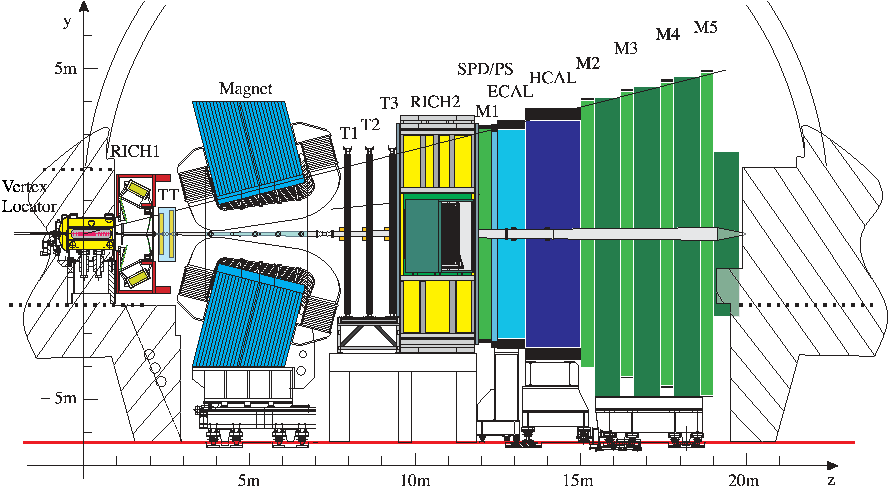
\includegraphics[width=0.8\textheight]{lhcb-detector-cross-section}
%  \caption[Cross-section view of \LHCb, cut in the non-bending $y$--$z$ plane]%
%    {Cross-section view of \LHCb, cut in the non-bending $y$--$z$ plane.}
%  \label{fig:LHCbCrossSection}
%  \end{center}
%\end{sidewaysfigure}



\chapter{The T2K Experiment}
\label{chap:T2KExperiment}
\begin{figure}
  \centering
  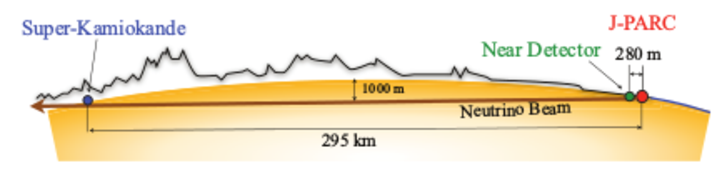
\includegraphics[width=10cm]{images/t2k/t2k_schematic.pdf}
  \caption{The T2K experiment.}
  \label{fig:T2KSchematic}
\end{figure}


The Tokai-to-Kamioka (T2K) experiment~\cite{Abe2011106} is a long baseline neutrino oscillation experiment located in two sites across Japan which was designed to study the parameters governing the PMNS matrix.  The first site is the J-PARC facility in Tokai-mura on Japan's east cost which houses a 30 GeV proton accelerator complex that is used to generate a highly pure $\nu_\mu$ beam.  J-PARC also contains a suite of detectors designed to measure the neutrino beam's unoscillated characteristics.  Super-Kamiokande (SK) is located 295 km (see Fig.~\ref{fig:T2KSchematic}) and measures the contents of the neutrino beam post-oscillation.
\newline
T2K was the first experiment to observe the $\nu_\mu\rightarrow\nu_e$ appearance channel~\cite{PhysRevLett.112.061802} which excluded $\theta_{13} = 0$ at 7.3$\textrm{\sigma}$ significance.  By comparing this result with precise $\theta_{13}$ measurements from reactor experiments, $\textrm{\delta}_{\textrm{CP}}$ regions can be excluded at 90$\%$ confidence level (see Fig.~\ref{fig:NueAppearanceContour}).  T2K's precision analysis of the $\nu_\mu$ disappearance channel provide world leading measurements of $\textrm{\theta}_{23}$ and $\Delta m^2_{23}$.  Independently of the oscillation analyses performed by the experiment, T2K's near detectors, ND280 and INGRID, are used to measure a range of neutrino cross-sections~\cite{PhysRevLett.113.241803, PhysRevD.87.092003}.  While this is not the primary aim of T2K, such measurements are still extremely important as T2K systematic uncertainties can be constrained with additional cross-section knowledge as well as helping to understand the general neutrino interaction picture.

\begin{figure}
  \centering
  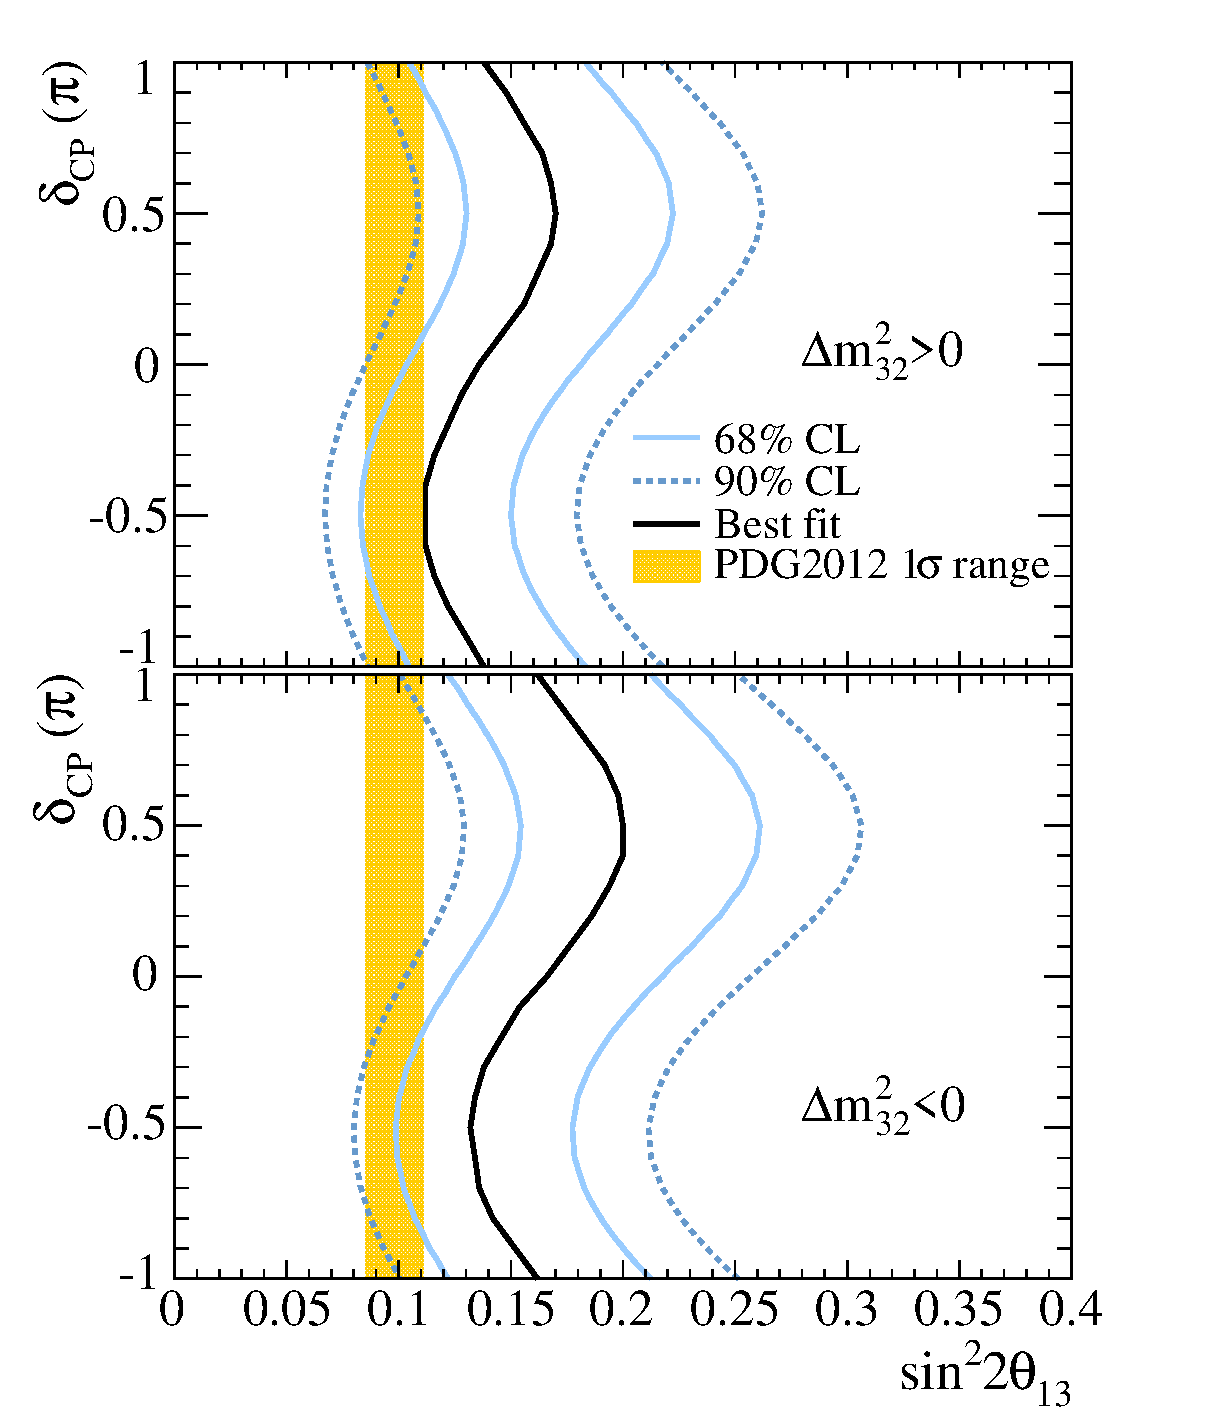
\includegraphics[width=7.5cm]{images/t2k/nue_appearance_Theta13Delta_contour.eps}
  \caption{The 68$\%$ and 90$\%$ confidence level allowed regions for $\sin^22\theta_{13}$ as a function of $\textrm{\delta}_{\textrm{CP}}$ for normal hierachy (top) and inverted hierarchy (bottom)  The solid line represents the best fit $\sin^22\theta_{13}$ for a given $\textrm{\delta}_{\textrm{CP}}$.  The shaded region shows the average $\theta_{13}$ provided by the reactor constraint~\cite{PhysRevLett.112.061802}.}
  \label{fig:NueAppearanceContour}
\end{figure}


\section{Accelerator complex}
\label{sec:AcceleratorComplex}
The T2K neutrino beam is generated by J-PARC's accelerator complex which produces a 30 GeV proton beam which is fired at a fixed graphite target.  The final states particles of the target interaction are predominately charged pions which decay to produce the neutrino beam.  Surrounding and behind the graphite target are a set of magnetic horns which focus the pions into a beam, resulting in a focused neutrino beam after the hadrons have decayed.

\subsection{Proton Accelerators}
\label{subsec:ProtonAccelerators}
Stuff about the accelerator

\subsection{Neutrino beamline}
\label{subsec:NeutrinoBeamline}
Stuff about the beamline

\section{Near detector complex}
\label{sec:NearDetectorComplex}
Stuff about comples

\subsection{Multi-Pixel Photon Counter}
\label{subsec:MPPC}
MPPCs

\subsection{INGRID}
\label{subsec:INGRID}
Stuff about INGRID

\subsection{ND280}
\label{subsec:ND280}
ND280 time

\subsubsection{The fine grain detectors}
\label{subsubsec:FGD}
FGDS

\subsubsection{The time projection chambers}
\label{subsubsec:TPC}
TPCs

\subsubsection{The $\pi^0$ detector}
\label{subsubsec:pi0detector}
Here is ref for \ref{subsubsec:TPC}
pi0

\subsubsection{The electromagnetic calorimeters}
\label{subsubsec:ecal}
The beasts

\subsubsection{The side muon range detector}
\label{subsubsec:smrd}
Why bother?

\subsection{The far detector}
I mean SK



